\documentclass{article}
\usepackage{ijcai15}

\usepackage{times}
%\usepackage{helvet}
%\usepackage{courier}
%\usepackage{xcolor}
\usepackage{longtable,multirow,colortbl,booktabs}
\usepackage{url}
%\usepackage{balance}
\usepackage{amsmath,amssymb, amsthm}
\newtheorem{theorem}[section]{Theorem}
\newtheorem{lemma}[section]{Lemma}
\newtheorem{definition}[section]{Definition}
\newtheorem{proposition}[section]{Proposition}
\usepackage{bm}

\newcommand{\st}{\mathrm{s.t.}}
\newcommand{\diag}{\mathrm{diag}}
\newcommand{\tr}{\mathrm{tr}}

\usepackage{algorithm,algorithmic}
\renewcommand{\algorithmicrequire}{\textbf{Input:}}
\renewcommand{\algorithmicensure}{\textbf{Output:}}
\renewcommand{\algorithmicreturn}{\textbf{Initialization:}}
\usepackage{threeparttable}
\usepackage{graphicx}
\usepackage{subfigure}


\pdfinfo{
/Title (Robust Multiple Kernel K-means using L21-norm)
/Author (Liang Du, Peng Zhou, Lei Shi, Hanmo Wang, Mingyu Fan, Wenjian Wang, Yi-Dong Shen)
}


\title{Robust Multiple Kernel K-means using $\ell_{2,1}$-norm}
\author{Liang Du$^{1,2}$, Peng Zhou$^{1,3}$, Lei Shi$^{1,3}$, Hanmo Wang$^{1,3}$, Mingyu Fan$^{4}$, Wenjian Wang$^{2}$\thanks{Wenjian Wang is also affiliated with the Key Laboratory of Computational Intelligence and Chinese Information Processing of Ministry of Education, Shanxi University}, Yi-Dong Shen$^{1}$\thanks{Corresponding Author} \\
$^{1}$State Key Laboratory of Computer Science, Institute of Software, Chinese Academy of Sciences\\
$^{2}$School of Computer and Information Technology, Shanxi University \\
$^{3}$University of Chinese Academy of Sciences \\
$^{4}$Institute of Intelligent System and Decision, Wenzhou University\\
\{duliang,zhoup,ydshen\}@ios.ac.cn, fanmingyu@amss.ac.cn, wjwang@sxu.edu.cn
}


\begin{document}
\maketitle

\begin{abstract}
The k-means algorithm is one of the most often used method for data clustering. However, the standard k-means can only be applied in the original feature space. The kernel k-means, which extends k-means into the kernel space, can be used to capture the non-linear structure and identify arbitrarily shaped clusters. Since both the standard k-means and kernel k-means apply the squared error to measure the distances between data points and cluster centers, a few outliers will cause large errors and dominate the objection function. Besides, the performance of kernel method is largely determined by the choice of kernel. Unfortunately, the most suitable kernel for a particular task is often unknown in advance. In this paper, we first present a robust k-means using $\ell_{2,1}$-norm in the feature space and then extend it to the kernel space. To recap the powerfulness of kernel methods, we further propose a novel robust multiple kernel k-means (RMKKM) algorithm that simultaneously finds the best clustering label, the cluster membership and the optimal combination of multiple kernels. An alternating iterative schema is developed to find the optimal value. Extensive experiments well demonstrate the effectiveness of the proposed algorithms.
\end{abstract}


\section{Introduction}
Clustering is one of the most important research topics in both machine learning and data mining communities. It aims at partitioning the data points into groups with similar objects. An enormous number and variety of methods have been proposed over the past decades. Due to the simplicity and the effectiveness, the k-means algorithm \cite{wu2008top} becomes one of the most commonly-used methods for data clustering. However, the standard k-means algorithm is limited to the squared Euclidean distance and cannot identify arbitrarily shaped clusters.

Kernel clustering algorithms have the ability to capture the non-linear structure inherent in many real world data sets and thereby usually achieve better clustering performance. The typical kernel-based clustering methods include: kernel k-means \cite{scholkopf1998nonlinear} and spectral clustering \cite{ng2002spectral}. Efforts have been made to further improve the result of kernel k-means. \cite{dhillon2007weighted} shows that the spectral clustering can be equivalently reformulated as a weighted variant of kernel k-means. \cite{yu2012optimized} and \cite{huang2012multiple} propose to integrate multiple information for clustering. \cite{chitta2011approximate}, \cite{chitta2012efficient} and \cite{elgohary2014Embd} develop efficient optimization schema to improve the scalability of kernel k-means to hanle large scale data.

Although kernel k-means based methods have attracted increasing attention in recent years, they still suffer from the following problems in real applications. First, these methods adopt the squared loss, which is well-known to be unstable with respect to outliers and noises, to measure the reconstruction error. As a result, a few noisy entries with large errors may easily dominate the result. Second, it is known that the performance of these single kernel methods are largely determined by the choice of kernel. Unfortunately, the most suitable kernel for a particular task is often unknown in advance. Moreover, exhaustive search on a user-defined pool of kernels will be quite time-consuming when the size of the pool becomes large \cite{zeng2011feature}. In addition, real world data sets are often generated from different sources equipped with heterogeneous features. However, single kernel methods may fail to fully utilize such information. By leveraging multiple input kernels from different views or sources,  multiple kernel methods are with great potential to integrate complementary information \cite{yu2012optimized}. To alleviate the effort for kernel designing and make full use of complementary information, it is imperative to learn an appropriate kernel efficiently to make the performance of the kernel k-means robust or even improved. However, unlike the multiple kernel learning in supervised setting \cite{gonen2011multiple}, kernel learning in unsupervised scenario is more challenging due to the absence of class labels that could guide the search for relevant kernels.

To improve the robustness with respect to noises and outliers, we first propose a robust k-means method by using $\ell_{2,1}$-norm to measure the distances between data points and cluster centers. To recap the powerfulness of kernel method, we also provide the robust k-means in kernel space. To alleviate the effort of kernel construction and make use of complementary information, we further propose a robust multiple kernel k-means (RMKKM) algorithm. In particular, RMKKM performs robust k-means with an appropriate consensus kernel learned from a linear combination of multiple input kernels. To solve the optimization problem where all the variables are encapsulated by the non-smooth $\ell_{2,1}$-norm, an alternating iterative algorithm is provided to find the optimal value. Experimental results on benchmark data sets have shown that the proposed approaches achieve better clustering results in both the single kernel and multiple kernel learning settings.

The rest of the paper is organized as follows. The robust multiple kernel k-means is introduced in Section 2. Section 3 provides the optimization schema. A variety of experimental results are presented in Section 4. Finally, we provide some concluding remarks in Section 5.


\textbf{Notations.}  In this paper, matrices are written as uppercase letters and vectors are written as boldface lower-case letters. Given a matrix $A = \{a_{ij}\}$, we denote its $i$-th column as $\bm{a}_i$. The $\ell_2$-norm of a vector $\bm{x}$ is defined as $||\bm{x}||_2 = \sqrt{\bm{x}^T \bm{x}}$. The $\ell_{2,1}$-norm of a matrix is defined as $||A||_{2,1} = \sum_{i=1}^{n}\sqrt{\sum_{j=1}^{m} a_{ij}^2} = \sum_{i=1}^{n} ||\bm{a}_i||_2$.

\section{Robust Multiple Kernel K-means}
In this section, we first present the robust k-means using the $\ell_{2,1}$-norm. Then we extend it to kernel space and get robust multiple kernel k-means. To improve the effectiveness of kernel method, we further propose a novel robust multiple kernel k-means (RMKKM) algorithm for data clustering.
\subsection{Robust K-means}
Suppose we are given a data set $X = [\bm{x}_1, \bm{x}_2, \cdots, \bm{x}_n] \in \mathcal{R}^{d \times n} $, and aim to partition these data points into $c$ disjoint clusters $\{\mathcal{C}_1, \mathcal{C}_2, \ldots, \mathcal{C}_c\}$. The k-means algorithm finds optimal solutions with respect to the clustering error, defined as the sum of squared Euclidean distance between each data point $\bm{x}_i$ and the cluster center $\bm{u}_j$ where $\bm{x}_i$ belongs to. The objective function of k-means can be written as
\begin{align}\label{km_obj}
	\min_{Z,U} \quad & ||X - U Z^T||_2^2 \\
	\st \quad & z_{ij} = \{0, 1\}, \sum_{j=1}^{c} z_{ij} = 1, \forall i=1,2,\cdots,n, \nonumber
\end{align}
where $U \in \mathcal{R}^{d \times c}$ is the cluster centroid matrix, and $Z \in \mathcal{R}^{n \times c}$ is the cluster indicator matrix.

Though the k-means algorithm has been widely used for data clustering, it is known that the squared loss used in Eq. \eqref{km_obj} is very sensitive to data outliers, and they greatly affect the performance of clustering. In order to have a more stable result with respect to a fixed initialization, the robust k-means algorithm is desired. Inspired by the recent developed robust multi-view k-means \cite{cai2013multi}, we also use the $\ell_{2,1}$-norm to measure the reconstruction error, and get the following problem
\begin{align}\label{l21_km_obj}
	\min_{Z,U} \quad& ||X^T - Z U^T||_{2,1} = \sum_{i=1}^{n} \sqrt{\sum_{j=1}^{c}z_{ij}||\bm{x}_i - \bm{u}_j||^2} \\
\st \quad& z_{ij} = \{0, 1\}, \sum_{j=1}^{c} z_{ij} = 1, \forall i=1,2,\cdots,n, \nonumber
\end{align}
where the $\ell_{1}$-norm is imposed among data points and the $\ell_{2}$-norm is used for features. By introducing the sparsity induced norm, $\ell_{2,1}$-norm, the effects of data outliers can be reduced and a more robust result is expected.

\subsection{Robust Kernel K-means}
The effectiveness of k-means is largely limited to spherical clusters, that is, the clusters must be linearly separable \cite{dhillon2004kernel}. By applying kernel trick, the kernel k-means \cite{scholkopf1998nonlinear} algorithm attempts to address this problem by mapping data with non-linear transformation into appropriate feature space and applying k-means on the induced feature space. This can lead to linear separated clusters in the new feature space while these clusters are not linear separable in the original space. Thus, kernel k-means is much preferred for general clusteringn \cite{bishop2006pattern}.

Similar to the kernel k-means algorithm, the proposed robust k-means in Eq. \eqref{l21_km_obj} can also be easily extended to the kernel version by using a general kernelization framework \cite{zhang2010general}. Let $\phi : \mathcal{R}^{d} \rightarrow \mathcal{H}$ be a kernel mapping from the original space to the kernel space, where $\mathcal{H}$ is a Reproducing Kernel Hilbert Space (RKHS) induced by a kernel function $\mathcal{K}(\bm{x}, \bm{z}) = \phi(\bm{x})^T \phi(\bm{z})$. Then $\phi(X) = [\phi(\bm{x}_1), \phi(\bm{x}_2), \cdots, \phi(\bm{x}_n)]$, and the robust k-means in Eq. \eqref{l21_km_obj} in the kernel space becomes:
\begin{align}\label{l21_kkm}
     \min_{Z,V} \quad  &||\phi(X)^T - Z  V^T||_{2,1} \\
   =& \sum_{i=1}^{n}\sqrt{\sum_{j=1}^{c}z_{ij}||\phi(\bm{x}_i) - \bm{v}_j||^2}, \nonumber
\end{align}
where $V$ is the cluster center matrix in the implicit feature space. It can be shown later (see Eq. \eqref{v_update}), the $j$-th cluster center $\bm{v}_j$ can be determined by $\bm{v}_j = \sum_{i} a_{ij} \phi(\bm{x}_i)$, where $a_{ij}$ is the membership of $\bm{x}_i$ belongs to $j$-th cluster. Hence, the above problem can be re-written as
\begin{align}\label{rkkm}
    \min_{Z,A} \quad & \sum_{i=1}^{n} \sqrt{\sum_{j=1}^{c} z_{ij} (k_{ii} - 2 \bm{a}_{j}^{T} \bm{k}_{i}  + \bm{a}_{j}^{T} K \bm{a}_{j})},
\end{align}
where the kernel matrix is denoted by $K \in \mathcal{R}^{n \times n}$ and the $(i,j)$-th entry of $K$ is $k_{ij} = \phi(\bm{x}_i)^T \phi(\bm{x}_j)$.

\subsection{Robust Multiple Kernel K-means}
The proposed method above only works for single kernel data clustering. However, one of the central problems with kernel methods in general is that it is often unclear which kernel is the most suitable for a particular task. In this subsection, we further extend the above method to automatically learn an appropriate kernel from the convex linear combination of several pre-computed kernel matrices within the multiple kernel learning framework \cite{gonen2011multiple}.

Suppose there are altogether $m$ different kernel functions $\{\mathcal{K}\}_{t=1}^{m}$ available for the clustering task in hand. Accordingly, there are $m$ different associated feature spaces denoted as $\{\mathcal{H}\}_t^m$. To combine these kernels and also ensure that the resulted kernel still satisfies Mercer condition, we consider a nonnegative combination of these feature maps, $\phi'$ , that is,
\begin{align}
\phi'(\bm{x}) = \sum_{t=1}^{m} w_t \phi_t(\bm{x}) \quad \text{ with } w_t \geq 0.
\end{align}
Unfortunately, as these implicit mappings do not necessarily have the same dimensionality, such a linear combination may be unrealistic.
Hence, we construct an augmented Hilbert space $\mathcal{\tilde{H}} = \oplus_{t=1}^{m} \mathcal{H}^i$ by concatenating all feature spaces $\tilde{\phi}(\bm{x}) = [ \sqrt{w_1} \phi_{1}(\bm{x}); \sqrt{w_2} \phi_{2}(\bm{x}); \ldots; \sqrt{w_m} \phi_{m}(\bm{x}) ]^T$ with different weight $\sqrt{w_t}(w_t \geq 0)$ ,  or
equivalently the importance factor for kernel function $\mathcal{K}^t$. It can be verified that clustering in feature space $\mathcal{\tilde{H}}$ is equivalent to employing a combined kernel function \cite{zeng2011feature}
\begin{align}
\tilde{\mathcal{K}}(\bm{x}, \bm{z}) = \sum_{t=1}^{m} w_t \mathcal{K}^{t}(\bm{x}, \bm{z}).
\end{align}

It is known that the convex combination, with $\bm{w} (w_t \geq 0)$, of the positive semi-definite kernel matrices $\{ K\}_{t=1}^{m}$ is still a positive semi-definite kernel matrix. By replacing the single kernel in Eq. \eqref{rkkm} with the combined kernel, we propose a new Robust Multiple Kernel k-means method by solving:
\begin{align}\label{rmkkm}
    \min_{Z,A,\bm{w}}  \quad&  \sum_{i=1}^{n} \sqrt{\sum_{j=1}^{c} z_{ij}[\sum_{t=1}^{m} w_t( k_{ii}^{t} - 2 \bm{a}_j^T \bm{k}_i^t + \bm{a}_j^T K^t \bm{a}_j )]} \nonumber \\
    =& \sum_{i=1}^{n} \sqrt{\sum_{j=1}^{c} z_{ij}(\tilde{k}_{ii} - 2 \bm{a}_j^T \tilde{\bm{k}}_i + \bm{a}_j^T \tilde{K} \bm{a}_j )} \\
    \st  \quad&z_{ij} = \{0, 1\}, \sum_{j=1}^{c} z_{ij} = 1, \sum_{t=1}^{m} w_t^{\gamma} = 1, w_t \geq 0, \nonumber
\end{align}
where $\gamma$ is the parameter to control the kernel weight distribution with $0 < \gamma < 1$. It should be noticed that RMKKM aims at improving the stability of kernel k-means without suffering the choice of appropriate kernel functions, where the weak kernels can be computed either on single view or multi-view data \cite{cai2013multi}.
\section{Optimization Algorithm and Analysis}
The optimization problem in Eq. \eqref{rmkkm} is not convex in all variables together, but convex in them separately. The difficulty of solving the proposed objective mainly lies that all variables are encapsulated into a non-smooth $\ell_{2,1}$-norm. In the following, we introduce an iterative algorithm based on block coordinate descent to solve it. We separately update the value of $A,Z$, and $\bm{w}$ while holding the other variables as constant. Thus, a local minima can be expected by solving a sequence of convex optimization problems.

\subsection{Optimizing w.r.t. cluster centroid when $Z$ and $\bm{w}$ are fixed}
Recall that, we have introduced cluster centroid matrix $V$ in the implicit feature space in Eq. \eqref{l21_kkm}, conceptually we further denote $\tilde{\bm{v}}_j$ to be the concatenated implicit representations for $j$-th cluster center. The optimization problem in Eq. \eqref{rmkkm} with respect to the cluster centroid matrix can be re-written as
\begin{align}
	\mathcal{J}(\tilde{V}) = \sum_{i=1}^{n} \sqrt{ \sum_{j=1}^{c} z_{ij} ||\tilde{\phi}(\bm{x}_i) - \tilde{\bm{v}_j}||^2}.
\end{align}
It can be verified that the derivative of $\mathcal{J}$ is equivalent to the derivative of the following proxy function $\mathcal{L}(\tilde{V})$,
\begin{align}\label{w_kkm}
  \mathcal{L}(\tilde{V}) &= \sum_{i=1}^{n} D_{ii} \sum_{j=1}^{c} z_{ij}(\tilde{\phi}(\bm{x}_i) - \tilde{\bm{v}}_j)^2,
\end{align}
where $D_{ii}=\frac{1}{2\sqrt{ \sum_{j=1}^{c} z_{ij} ||\tilde{\phi}(\bm{x}_i) - \tilde{\bm{v}}_j||^2}}$, conceptually.

Actually, the above problem is the weighted version of kernel k-means \cite{dhillon2004kernel}. By setting the derivative to be zero, we have
\begin{align}
  \frac{\partial \mathcal{L} }{\partial \bm{v}_j} &= -2\sum_{i=1}^{n}z_{ij}(\tilde{\phi}(\bm{x}_i) - \tilde{\bm{v}}_j) = 0.
\end{align}
\begin{align}\label{v_update}
  \bm{v}_j &= \frac{\sum_{i=1}^{n}z_{ij} D_{ii} \tilde{\phi}(\bm{x}_i)}{\sum_{i=1}^{n}z_{ij} D_{ii}}.
\end{align}
Thus, it is clear that the cluster centroid matrix for robust (multiple) kernel k-means can be determined by the weighted combination of the data in implicit feature space, where the membership matrix $A$ can be computed by
\begin{align}\label{update_a}
  a_{ij} = \frac{z_{ij} D_{ii} }{\sum_{i=1}^{n}z_{ij} D_{ii}}.
\end{align}
And the actual value of $D_{ii}$ can be computed by
\begin{align}\label{update_d}
  D_{ii} = \frac{1}{2\sqrt{\sum_{j=1}^{c}z_{ij}\sum_{t=1}^{m}w_t( k_{ii}^{t} - 2 \bm{a}_j^T \bm{k}_i^t + \bm{a}_j^T K^t \bm{a}_j )}}.
\end{align}
\subsection{Optimizing w.r.t. partition matrix $Z$ when $A$ and $\bm{w}$ are fixed}
The minimization of the objective function in Eq. \eqref{rmkkm} with respect to $Z$ can be decomposed into solving $n$ independent sub-problems, that is
\begin{align}
\min_{\bm{z}_i} \quad& \sqrt{\sum_{j=1}^{c} z_{ij}(\tilde{k}_{ii} - 2 \bm{a}_j^T \tilde{\bm{k}}_i + \bm{a}_j^T \tilde{K} \bm{a}_j )},
\end{align}
where $z_{ij} = \{0, 1\}, \sum_{j=1}^{c} z_{ij} = 1$.
And, the optimal solution of the above problem is given by
\begin{align}\label{update_z}
  z_{ij} \!=\! \left\{ \begin{array}{ll}
                     1 & j=\arg\min_{j'}(\sum_{t=1}^{m}w_t( \bm{a}_{j'}^T K^t \bm{a}_{j'}  \!-\! 2 \bm{a}_{j'}^T \bm{k}_i^t )) \\
                     0 & \textrm{otherwise.}
                   \end{array}
  \right.
\end{align}

\subsection{Optimizing w.r.t. kernel weight $\bm{w}$ when $A$ and $Z$ are fixed}
By defining $E \in \mathcal{R}^{n \times m}$ with
\begin{equation}
    e_{it} = \sum_{j=1}^{c} z_{ij} ( k_{ii}^{t} - 2 \bm{a}_j^T \bm{k}_i^t + \bm{a}_j^T K^t \bm{a}_j ),
\end{equation}
the optimization of Eq. \eqref{rmkkm} with respect to $\bm{w}$ can be simplified as solving the following problem
\begin{align}\label{w_obj}
	\min  \quad & \sum_{i=1}^{n} \sqrt{\sum_{t=1}^{m} \bm{w}_t e_{it}}, \quad \st \sum_{t=1}^{m} w_t^{\gamma} = 1, w_t \geq 0.
\end{align}
It is obvious that the derivative in Eq. \eqref{w_obj} can also be regarded as the derivative of the following objective function
\begin{align}\label{w_proxy}
\mathcal{L}(\bm{w}) = \sum_{t=1} w_t h_t ,\quad \st \quad \sum_{t=1}^{m} w_t^{\gamma} = 1, w_t \geq 0,
\end{align}
where $h_t$ is denoted as
\begin{align}\label{w_grad}
h_t =\sum_{i=1}^{n} \frac{e_{it}}{2 \sqrt{\sum_{t'=1}^{m} w_{t'} e_{it'}} }.
\end{align}
The Lagrange function of Eq. \eqref{w_proxy} is $\mathcal{J}(\bm{w}) = \bm{w}^T \bm{h} + \lambda (1 - \sum_{t}w_t^{\gamma})$.
By using the KKT condition $\frac{\partial \mathcal{J}(\bm{w})}{\partial w_t} w_ t= 0$ and the constraint $\sum_{t=1}^{m} w_t^{\gamma} = 1$, the optimal solution of $\bm{w}$ can be obtained by
\begin{align}\label{update_w}
  w_t = \left[ \frac{1}{\sum_{t'=1}^{m} h_{t'}^{\frac{\gamma}{\gamma - 1}}}\right]^\frac{1}{\gamma} h_{t}^{\frac{1}{\gamma -1}}.
\end{align}

In summary, we present the alternating iterative algorithm for optimizing Eq. \eqref{rmkkm} in Algorithm \ref{rmkkm_alg}.
\begin{algorithm}
    \caption{The algorithm of RMKKM}
	\label{rmkkm_alg}
	\begin{algorithmic}
	\REQUIRE{A set of kernels $\{K^{t}\}_{t=1}^{m}$, the desired number of  cluster $c$ and the parameter $\gamma$.}
    \STATE{Initialize the indicator matrix $Z$ randomly, such that $Z$ satisfies $z_{ij}=\{0,1\}$ and $\sum_j z_{ij}=1$;}
    \STATE{Initialize the kernel weight $w_t = 1/m$ for each kernel;}
    \STATE{Initialize the diagonal matrix $D=I_{n}$, where $I_{n}$ is the identity matrix;}
	\REPEAT
	\STATE{Update the membership matrix $A$ by Eq. \eqref{update_a};}
	\STATE{Update the cluster indicator matrix $Z$ by Eq. \eqref{update_z};}
	\STATE{Update the kernel weight $\bm{w}$ by Eq. \eqref{update_w};}
	\STATE{Update the diagonal matrix $D$ by Eq. \eqref{update_d};}
	\UNTIL{Converges}
    \ENSURE{Partition matrix $Z$, membership matrix $A$, and the kernel weights $\bm{w}$.}
	\end{algorithmic}
  \end{algorithm}
\subsection{Convergence Analysis}
The optimization problem of Eq. \eqref{rmkkm} is a convex problem with respect to one variable while holding the others. For each subproblem, our algorithm will guarantee that we can find the optimal solution.
Therefore, by solving these subproblems alternatively, our algorithm will reduce the objective function monotonically. Meanwhile, the whole problem is lower bounded. Thus, the convergence of the proposed algorithm can be verified.

\subsection{Complexity Analysis}
In the following, we give the complexity analysis of the optimization algorithm. Initially, we need to compute the $n \times n \times m$ kernel matrices $\{K\}_{t=1}^{m}$, whose cost is generally $O(n^2dm)$. In each iteration, the cost of updating $A$ by Eq. \eqref{update_a} is $O(nc)$, the cost of updating $Z$ by Eq. \eqref{update_z} is $O((n^2+n)cm)$, the cost of updating $\bm{w}$ by Eq. \eqref{update_w} is $O((n^2+n)nm + nm + m)$, and the cost of updating $D$ by Eq. \eqref{update_d} is $O((n^2+n)nm)$. Since $c \ll n$, the total cost is $O(n^2dm + (n^3 + n^2 + n)ml)$, where $l$ is the number of iterations. Compared with kernel k-means with fixed kernel weights and sample weights, the proposed algorithm is less efficient due to the involvement of updating kernel weight $\bm{w}$ and sample weight $D$.
\subsection{Discussion of the parameter $\gamma$}
The parameter $\gamma$ is used to control the distribution of weights for different kernels. From Eq. \eqref{update_w}, we can observe that
when $\gamma \rightarrow 1$, we will assign 1 to the kernel whose $h_t$ is the smallest and assign 0 to the weights of other kernels. And when $\gamma \rightarrow 0$, we will get equal weights.
With this strategy, we can avoid the trivial solution of the kernel weights $\bm{w}$ and control the whole weights distribution flexibly.
\section{Experimental Results}
In this section, we evaluate the clustering performance of the proposed algorithm on a number of real world data sets.

\subsection{Data Sets}
We collect a variety of data sets, including 6 image data sets and 3 text corpora, most of which have been frequently used to evaluate the performance of different clustering algorithms. The statistics of these data sets are summarized in Table \ref{data}.

\begin{table}[h]
\centering
\caption{Description of the data sets}
\label{data}
\begin{tabular}{|l|c|c|c|}
\hline
&\textrm{\# instances}&\textrm{\# features}&\textrm{\# classes}\\\hline
\textrm{YALE}&165&1024&15\\\hline
\textrm{JAFFE}&213&676&10\\\hline
\textrm{ORL}&400&1024&40\\\hline
\textrm{AR}&840&768&120\\\hline
\textrm{COIL20}&1440&768&20\\\hline
\textrm{BA}&1404&320&36\\\hline
\textrm{TR11}&414&6429&9\\\hline
\textrm{TR41}&878&7454&10\\\hline
\textrm{TR45}&690&8261&10\\\hline
\end{tabular}
\end{table}

\begin{table*}[!htb]
\centering
\caption{Clustering results measured by Accuracy/NMI/Purity of the compared methods.}
\label{table:res_aio}
\setlength{\tabcolsep}{2.0pt}
\begin{tabular}{l c c c c c c c c c c c c c c}
        \toprule
        \small{Data} & \small{Metrics} & \small{KKM-b} & \small{KKM-a} & \small{SC-b} & \small{SC-a} & \small{RKKM-b} & \small{RKKM-a} & \small{KKM-ew} & \small{SC-ew} & \small{RKKM-ew}& \small{MKKM} & \small{AASC} & \small{RMKKM}$^*$ \\
        \midrule
        \multirow{3}{*}{\small{YALE}} & Acc & 0.4712&0.3897&\textbf{0.4942}&0.4052&0.4809&0.3971&0.4100&0.4973&0.4106&0.4570&0.4064&\textbf{0.5218}\\
		& NMI & 0.5134&0.4207&\textbf{0.5292}&0.4479&0.5229&0.4287&0.4571&0.5326&0.4601&0.5006&0.4683&\textbf{0.5558}\\
		& Purity &0.4915&0.4112&\textbf{0.5161}&0.4306&0.4979&0.4174&0.4345&0.5148&0.4358&0.4752&0.4233&\textbf{0.5364}\\
		\midrule
		\multirow{3}{*}{\small{JAFFE}} & Acc & 0.7439&0.6709&0.7488&0.5403&\textbf{0.7561}&0.6798&0.6254&0.5376&0.6277&0.7455&0.3035&\textbf{0.8707}\\
		& NMI & 0.8013&0.7148&0.8208&0.5935&\textbf{0.8347}&0.7401&0.6962&0.5913&0.7017&0.7979&0.2722&\textbf{0.8937}\\
		& Purity & 0.7732&0.7013&0.7683&0.5656&\textbf{0.7958}&0.7182&0.6655&0.5643&0.6683&0.7683&0.3308&\textbf{0.8890}\\
		\midrule
        \multirow{3}{*}{\small{ORL}} & Acc & 0.5353&0.4593&\textbf{0.5796}&0.4665&0.5496&0.4688&0.4726&0.4810&0.4815&0.4751&0.2720&\textbf{0.5560}\\
		& NMI& 0.7343&0.6336&\textbf{0.7516}&0.6674&0.7423&0.6391&0.6757&0.6939&0.6845&0.6886&0.4377&\textbf{0.7483}\\
		& Purity & 0.5803&0.5042&\textbf{0.6145}&0.5120&0.5960&0.5146&0.5189&0.5233&0.5285&0.5140&0.3156&\textbf{0.6023}\\
		\midrule
        \multirow{3}{*}{\small{AR}} & Acc & 0.3302&0.3089&0.2883&0.2222&\textbf{0.3343} &0.3120&0.3185&0.2188&0.3184&0.2861&0.3323&\textbf{0.3437}\\
		& NMI & 0.6521&0.6064&0.5837&0.5605&\textbf{0.6544} &0.6081&0.6334&0.5805&0.6334&0.5917&0.6506&\textbf{0.6549}\\
		& Purity & 0.3552&0.3364&0.3324&0.2599&\textbf{0.3587} &0.3388&0.3464&0.2533&0.3464&0.3046&0.3498&\textbf{0.3678} \\
		\midrule
        \multirow{3}{*}{\small{COIL20}} & Acc & 0.5949&0.5074&\textbf{0.6770}&0.4365&0.6164&0.5189&0.5483&0.3694&0.5543&0.5482&0.3487&\textbf{0.6665}\\
		& NMI &0.7405&0.6357&\textbf{0.8098}&0.5434&0.7463&0.6370&0.7072&0.4647&0.7098&0.7064&0.4187&\textbf{0.7734}\\
		& Purity & 0.6461&0.5530&\textbf{0.6992}&0.4683&0.6635&0.5634&0.5945&0.3980&0.6012&0.5895&0.3914&\textbf{0.6995}\\
		\midrule
        \multirow{3}{*}{\small{BA}} & Acc & 0.4120&0.3366&0.3107&0.2625&\textbf{0.4217}&0.3435&0.3637&0.2902&0.3699&0.4052&0.2707&\textbf{0.4342}\\
        & NMI &0.5725&0.4649&0.5076&0.4009&\textbf{0.5782}&0.4691&0.5228&0.4438&0.5293&0.5688&0.4234&\textbf{0.5847}\\
        & Purity & 0.4420&0.3606&0.3450&0.2907&\textbf{0.4528}&0.3686&0.3876&0.3206&0.3946&0.4347&0.3029&\textbf{0.4627}\\
        \midrule
        \multirow{3}{*}{\small{TR11}} & Acc & 0.5191&0.4465&0.5098&0.4332&\textbf{0.5303}&0.4504&0.4382&0.4651&0.4384&0.5013&0.4715&\textbf{0.5771}\\
		& NMI & 0.4888&0.3322&0.4311&0.3139&\textbf{0.4969}&0.3348&0.3504&0.3814&0.3506&0.4456&0.3939&\textbf{0.5608}\\
		& Purity & 0.6757&0.5632&0.5879&0.5023&\textbf{0.6793}&0.5640&0.5825&0.5464&0.5826&0.6548&0.5467&\textbf{0.7293}\\
		\midrule
		\multirow{3}{*}{\small{TR41}} & Acc & 0.5564&0.4634&\textbf{0.6352}&0.4480&0.5676&0.4680&0.4755&0.4723&0.4784&0.5610&0.4590&\textbf{0.6265}\\
		& NMI & 0.5988&0.4037&\textbf{0.6133}&0.3660&0.6077&0.4086&0.4245&0.4362&0.4292&0.5775&0.4305&\textbf{0.6347}\\
		& Purity & 0.7446&0.6000&0.7368&0.5645&\textbf{0.7499}&0.6021&0.6367&0.6269&0.6395&0.7283&0.6205&\textbf{0.7757}\\
		\midrule
		\multirow{3}{*}{\small{TR45}} & Acc & \textbf{0.5879}&0.4558&0.5739&0.4596&0.5813&0.4569&0.4512&0.5329&0.4530&0.5846&0.5264&\textbf{0.6400}\\
		& NMI & \textbf{0.5787}&0.3869&0.4803&0.3322&0.5786&0.3896&0.4022&0.4198&0.4057&0.5617&0.4194&\textbf{0.6273}\\
		& Purity & \textbf{0.6849}&0.5364&0.6125&0.5002&0.6818&0.5375&0.5586&0.5697&0.5604&0.6914&0.5749&\textbf{0.7520}\\
		\midrule
		\multirow{3}{*}{\small{Average}} & mAcc & 0.5279&0.4487&0.5353&0.4082&\textbf{0.5376}&0.4550&0.4559&0.4294&0.4591&0.5071&0.3767&\textbf{0.5817}\\
		& mNMI & 0.6312&0.5110&0.6141&0.4695&\textbf{0.6402}&0.5172&0.5411&0.5049&0.5449&0.6043&0.4350&\textbf{0.6697}\\
		& mPurity & 0.5993&0.5074&0.5792&0.4549&\textbf{0.6084}&0.5139&0.5250&0.4797&0.5286&0.5734&0.4284&\textbf{0.6462}\\
		\bottomrule
\end{tabular}
\begin{tablenotes}
\item[*] $^*$ The parameter $\gamma$ for RMKKM is set to $0.3$ for all the data sets.
\end{tablenotes}
\end{table*}

\subsection{Compared Algorithms}
To demonstrate how the clustering performance can be improved by the proposed approaches, we compared the results of the following algorithms:
\begin{itemize}
  \item Single kernel methods. Since we have multiple input kernels in hand, we run Kernel K-means (KKM), Spectral Clustering (SC) \cite{ng2002spectral}, and Robust Kernel K-means (RKKM) in Eq. \eqref{rkkm} on each kernel separately. And both the best and the average results over all these kernels are reported, which are referred to KKM-b, KKM-a, SC-b, SC-a, RKKM-b, RKKM-a, respectively. Due to space limitation, the worst results for single kernel are not reported. It should be pointed out that the worst results are often far below the average.
  \item Equal weighted methods. The multiple input kernels are combined into a single kernel with equal weights, and then report the results of KKM-ew, SC-ew, RKKM-ew. Note that such strategy often gets more stable results in multiple kernel learning \cite{gonen2011multiple}.
  \item MKKM\footnote{\url{http://imp.iis.sinica.edu.tw/IVCLab/research/Sean/mkfc/code.rar}.}.
  The MKKM proposed in \cite{huang2012multiple} also extends k-means in multiple kernel setting. Both the loss function and the constraint on the kernel weight distribution are different to our method.
  \item AASC\footnote{\url{http://imp.iis.sinica.edu.tw/IVCLab/research/Sean/aasc/code.rar}.}.
  The AASC algorithm is proposed in \cite{huang2012affinity} for multiple affinities aggregation.
  \item RMKKM\footnote{For the purpose of reproducibility, we provide the code at \url{https://github.com/csliangdu/RMKKM}.}. The proposed robust multiple kernel k-means method for data clustering.
\end{itemize}

\subsection{Experiment Setup}
Following the similar strategy of other multiple kernel learning approaches, we apply 12 different kernel functions as basis for multiple kernel clustering. These kernels include, seven RBF kernels $\mathcal{K}(\bm{x}_i, \bm{x}_j) = \exp(-||\bm{x}_i -  \bm{x}_j||^2 /2 \delta^2)$ with $\delta = t * D_0$, where $D_0$ is the maximum distance between samples and $t$ varies in the range of $\{0.01, 0.05, 0.1, 1, 10, 50, 100\}$, four polynomial kernels $\mathcal{K}(\bm{x}_i, \bm{x}_j) = (a + \bm{x}_i^T \bm{x}_j)^b$ with $a = \{0, 1\}$ and $b = \{2, 4\}$ and a cosine kernel $\mathcal{K}(\bm{x}_i, \bm{x}_j) = (\bm{x}_i^T \bm{x}_j)/(||\bm{x}_i||\cdot|| \bm{x}||)$. Finally, all the kernels have been normalized through $\mathcal{K}(\bm{x}_i, \bm{x}_j) = \mathcal{K}(\bm{x}_i, \bm{x}_j)/\sqrt{\mathcal{K}(\bm{x}_i, \bm{x}_i)\mathcal{K}(\bm{x}_j, \bm{x}_j)}$ and then rescaled to $[0,1]$.

The number of clusters is set to the true number of classes for all the data sets and clustering algorithms. For SC and AASC, the discrete clustering result is obtained by running k-means on spectral embedding. For the proposed method RMKKM,  the parameter $\gamma$ to control the kernel weight distribution is set to 0.3. In addition, the results of all these compared algorithms depend on the initialization. As suggested in \cite{yang2010image}, we independently repeat the experiments for 20 times with random initializations and report the best results corresponding to the best objective values.

Three clustering evaluation metrics are adopted to measure the clustering performance, that is, Clustering Accuracy (Acc), Normalized Mutual Information(NMI) and Purity.

\subsection{Experimental Results}
Table \ref{table:res_aio} shows the clustering results in terms of accuracy, NMI and purity on all the data sets. Both the best results for single kernel methods and multiple kernel methods are highlighted in boldface. These experiments reveal a number of interesting points: 1)The performance of single kernel methods (the first 6 columns), i.e., KKM, SC, RKKM, is largely determined by the choice of kernel function. On the one hand, with proper kernel function, these methods usually present good results. On the other hand, their performances are significantly deteriorated on inappropriate kernels. Such observations also motivate the development of robust kernel k-means for multiple kernel learning. Besides, it can also be seen that the proposed RKKM give best results on 5 data sets with single input kernel. 2)Clustering on the equal weighted multiple kernel combination often gives more reasonable and reliable results. Thus, it could be expected that with much carefully designed kernel weighting schema, the performance of multiple kernel clustering can be further boosted. 3)With proper kernel weight learning schema, the multiple kernel clustering approaches usually improve the results over simple equally weighted combination. 4)The proposed RMKKM gives the best results on these data sets for multiple kernel clustering. The performance of RMKKM is usually better or close to the result on the best single kernel. Note that, RMKKM does not need perform exhaustive search on a predefined pool of kernels. Such results well demonstrate the superiority of our method.


\subsection{Parameter Selection}
Our proposed method RMKKM introduces the parameter $\gamma$ to control the kernel weight distribution. The effect of the parameter $\gamma$ has been discussed in previous section. Here, we evaluate it empirically. Figure \ref{fig:rmkkm_gamma} shows how the clustering result in terms of NMI varies with the parameter $\gamma$ on two image data sets, JAFFE and ORL, and two document data sets, TR11 and TR41.

As we can see, the performance of RMKKM is very stable with respect to the parameter $\gamma$. Compared with the average performance of single kernel method, i.e., KKM-a, and the result of equally weighted kernel fusion, i.e., KKM-ew, the RMKKM achieves consistently good performance when $\gamma$ varies from 0.3 to 0.9 on all four data sets.


\begin{figure}[ht]
\centering
\subfigure[]{\label{fig:jaffe_gamma} 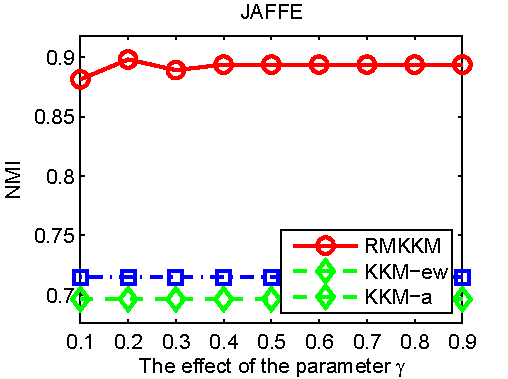
\includegraphics[width=0.23\textwidth]{gamma_jaffe_213n_676d_10c_uni_res}}
\hspace{-.25in}
\subfigure[]{\label{fig:orl_gamma} 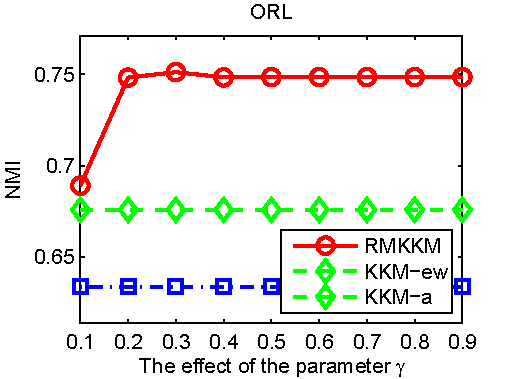
\includegraphics[width=0.24\textwidth]{gamma_ORL_400n_1024d_40c_zscore_uni_res} }

\subfigure[]{\label{fig:tr11_gamma} 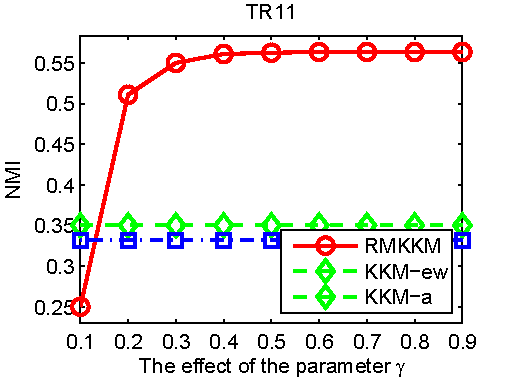
\includegraphics[width=0.23\textwidth]{gamma_tr11_414n_6429d_9c_tfidf_uni_res}}
\hspace{-.25in}
\subfigure[]{ \label{fig:tr41_gamma} 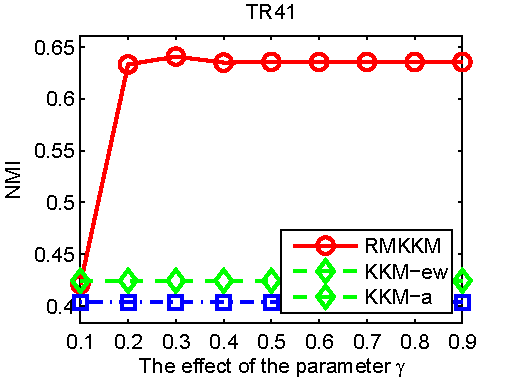
\includegraphics[width=0.23\textwidth]{gamma_tr41_878n_7454d_10c_tfidf_uni_res} }
\caption{The performance of RMKKM is stable with respect to the parameter $\gamma$.}
% \setlength{\abovecaptionskip}{1in}
\label{fig:rmkkm_gamma}
\end{figure}


\section{Conclusion}
In this paper, we presented a robust k-means method which uses $\ell_{2,1}$-norm to quantify the distances between data points and cluster centers. Then we extended it to perform robust k-means in the kernel space. To fully recap the powerfulness of kernel methods, we further proposed a robust multiple kernel k-means algorithm for clustering, i.e. RMKKM. It automatically learns an appropriate kernel from a lot of input kernels, which significantly reduces the effort of kernel designing or selection. Experimental results well demonstrate the superiority of the proposed method on benchmark data sets with multiple input kernels.

It has been shown that, given the kernel weight, the remained problem can be finally reformulated as a adaptively weighted kernel k-means (see Eq. \eqref{w_kkm}). Thus, in the future, we plan to investigate the use of the Nystr{\"o}m method \cite{elgohary2014Embd} and the random fourier feature \cite{yang2012nystrom} to make the proposed algorithms more efficient in terms of computational and memory complexity. Besides, we want to further investigate the effectiveness of the proposed method on multi-view and multi-source data clustering, where a bundle of input kernels is also available.
\section{Acknowledgments}
This work is supported in part by China National 973 program 2014CB340301 and NSFC grant 61379043, 61273291, 61203241, 61473212, Shanxi Scholarship Council of China (No.2012-008), Open Project Foundation of Information Technology Research Base of Civil Aviation Administration of China (No. CAAC-ITRB-201305).

\nocite{*}
\bibliographystyle{named}
\bibliography{rmkkm}
\end{document}
